% Figure 4 -- end-to-end walkthrough of one prospective node.
% Requires: \usepackage{graphicx}
% Regenerate with: python3 make_figure4.py
% Files: figure4_walkthrough.pdf  vector, 179.9 x 69.1 mm, selectable text
%        figure4_walkthrough.svg  source
%        figure4_walkthrough.png  640 dpi raster fallback

\begin{figure*}[tp]
  \centering
  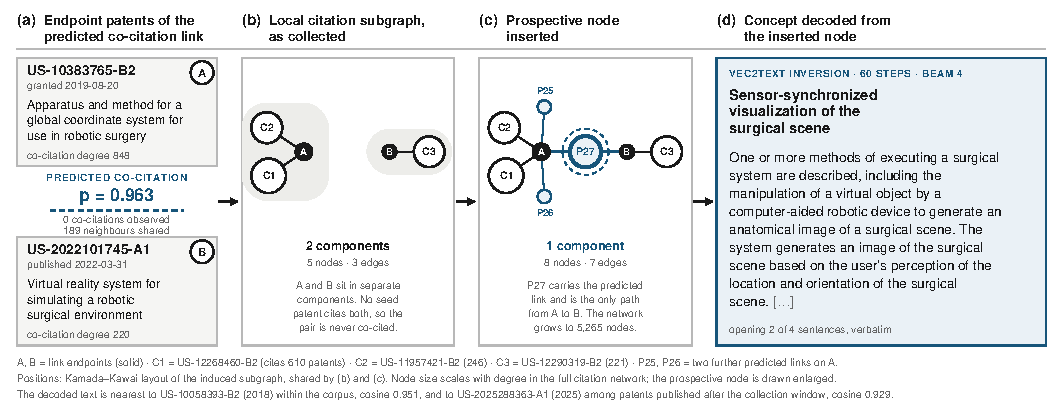
\includegraphics[width=\textwidth]{figure4_walkthrough.pdf}
  \caption{\textbf{End-to-end walkthrough of one prospective node.}
  Black marks what is present in the collected data, blue what the method
  synthesises.
  \textbf{(a)}~The two patents at the ends of predicted link row~26. They share
  189 co-citation neighbours, yet no document in the corpus cites both, so the
  pair carries no observed co-citation edge.
  \textbf{(b)}~Their local citation subgraph, exactly as collected: the induced
  one-hop neighbourhood of the pair is 5 nodes and 3 edges, and it falls into
  \emph{two} components (shaded), because the seed patents citing~A and the seed
  patent citing~B are different documents.
  \textbf{(c)}~The same subgraph after insertion. The prospective node carrying
  the predicted link joins the two components into one and is the only path from
  A to~B; across all 55 predicted links the citation network grows from 5{,}210
  to 5{,}265 nodes. Node positions are a Kamada--Kawai layout of the induced
  subgraph, computed once and shared by (b) and (c), so the two panels differ
  only by what insertion adds.
  \textbf{(d)}~The concept decoded from that node's projected embedding. A
  text-initialised GAT embeds the node from its new structural position, a
  ridge-plus-residual-MLP projection carries the embedding into the
  1{,}536-dimensional text-embedding space (round-trip cosine 0.967), and
  vec2text inverts it; the opening sentences are reproduced verbatim.
  Link row~26 is shown because its concept ranks first of all 55 in the
  subsequent-patent validation.}
  \label{fig:walkthrough}
\end{figure*}
